\documentclass[aspectratio=169]{beamer}

\usetheme{default}
\usecolortheme{whale}
\setbeamertemplate{navigation symbols}{}
\setbeamertemplate{footline}[frame number]
\setbeamerfont{title}{size=\large}
\setbeamerfont{frametitle}{size=\large}

\usepackage{amsmath,amssymb}
\usepackage{booktabs}
\usepackage{graphicx}

\graphicspath{{../paper/figures/}}

\title{Do Register Tokens Regularize Vision Transformers Under Data Scarcity?}
\subtitle{A controlled 12-run ablation on low-data CIFAR-100}
\author{Shahin \and Gulnisa \and Narmina \and Emil \and Rufet}
\institute{DLE-AI-202: Deep Learning, Cohort I 2026 --- Track 1: Pure Research}
\date{}

\begin{document}

\begin{frame}
\titlepage
\end{frame}

\begin{frame}{The question}
\textbf{Registers at scale.} Darcet et al.\ (ICLR 2024): large ViTs recycle a few
patch tokens as scratch space. Adding $K$ learnable \emph{register} tokens
removes the artifact.

\medskip
That was shown where there is \emph{too much} data to overfit.

\bigskip
\begin{block}{Our question}
When a ViT is starved of data, do registers reduce the generalization gap ---
and does any such reduction transfer to held-out performance?
\end{block}

\bigskip
\begin{columns}[T]
\column{0.33\textwidth}
\textbf{H1} Structural regularization: $\Delta\mathcal{L}$ falls.
\column{0.33\textwidth}
\textbf{H2} Capacity dilution: large $K$ hurts at $d=192$.
\column{0.33\textwidth}
\textbf{H3} Registers prevent attention-entropy collapse.
\end{columns}
\end{frame}

\begin{frame}{Design: one variable, twelve runs}
\begin{columns}[T]
\column{0.52\textwidth}
\textbf{Matrix.} $K \in \{0,1,4,8\} \times$ seeds $\{42, 1337, 3407\}$.

\medskip
\textbf{Data.} CIFAR-100, 100 images/class: 9{,}000 train / 1{,}000 val, plus
the untouched 10{,}000-image test split.

\medskip
\textbf{Model.} ViT-Tiny, $d=192$, 12 blocks, ImageNet-pretrained.
$K=8$ adds 1{,}536 of 5.54\,M parameters.

\medskip
\textbf{Budget.} 50 epochs, AdamW, cosine, AMP. 2.83 GPU-hours total.

\column{0.44\textwidth}
\begin{block}{What makes it a controlled test}
Within a seed, the subset, the split, the batch order and every
hyperparameter are identical across arms. $K$ is the only thing that moves.
\end{block}
\begin{block}{Why paired statistics}
At $n=3$, between-seed spread (2.17 pp) swamps any treatment effect. All
differences are formed \emph{within} a seed, then reduced.
\end{block}
\end{columns}
\end{frame}

\begin{frame}{Result 1: no arm improves held-out Top-1}
\begin{center}
\scriptsize
\setlength{\tabcolsep}{4pt}
\begin{tabular}{lcccc}
\toprule
\textbf{Configuration} & \textbf{Test Top-1 (\%)} & \textbf{Test Loss} & \textbf{Val Loss} & \textbf{Gap $\Delta\mathcal{L}$} \\
\midrule
Baseline ($K=0$)  & \textbf{75.19 $\pm$ 0.24} & \textbf{1.6357 $\pm$ 0.0018} & 1.6829 $\pm$ 0.0609 & 0.8047 $\pm$ 0.0628 \\
Registers ($K=1$) & 74.66 $\pm$ 0.42 & 1.6500 $\pm$ 0.0089 & 1.6545 $\pm$ 0.0380 & 0.7764 $\pm$ 0.0354 \\
Registers ($K=4$) & 75.06 $\pm$ 0.33 & 1.6375 $\pm$ 0.0117 & \textbf{1.6492 $\pm$ 0.0536} & \textbf{0.7680 $\pm$ 0.0514} \\
Registers ($K=8$) & 74.67 $\pm$ 0.12 & 1.6560 $\pm$ 0.0022 & 1.6602 $\pm$ 0.0268 & 0.7773 $\pm$ 0.0288 \\
\bottomrule
\end{tabular}
\end{center}

\bigskip
The bolding splits down the middle: the control wins both test columns, $K=4$
wins both validation-derived columns.

\medskip
Paired per seed: $K=1$ and $K=8$ lose accuracy in \textbf{3 of 3} seeds;
$K=4$ wins in 1 of 3 ($\bar\delta = -0.13$ pp, $p = 0.466$).

\medskip
Top-5 is the one place a register arm leads --- $K=4$ at $92.54 \pm 0.23$ vs
$92.43 \pm 0.14$ --- but paired it is $+0.11$ pp with SD $0.39$, 2/3 seeds,
$p = 0.681$.
\end{frame}

\begin{frame}{Result 2: H1 holds on validation and dies on test}
\begin{columns}[T]
\column{0.55\textwidth}

\includegraphics[width=\linewidth]{gen_gap_vs_registers.pdf}

\column{0.43\textwidth}
$K=4$ vs.\ control, paired over seeds:
\medskip

\footnotesize
\begin{tabular}{lrrr}
\toprule
& $\bar\delta$ & Dir. & $p$ \\
\midrule
Val loss  & $-0.0337$ & 3/3 & 0.024 \\
Gen.\ gap & $-0.0367$ & 3/3 & 0.051 \\
Test loss & $+0.0018$ & 2/3 & 0.823 \\
\bottomrule
\end{tabular}

\medskip
\normalsize
\textbf{Why it dies:} final training loss is 0.8782 / 0.8780 / 0.8812 / 0.8829
across $K = 0,1,4,8$ --- a spread of 0.005.

A regularizer trades training fit for held-out fit. Nothing was traded.
\end{columns}
\end{frame}

\begin{frame}{Why the validation split misled us}
\begin{columns}[T]
\column{0.55\textwidth}
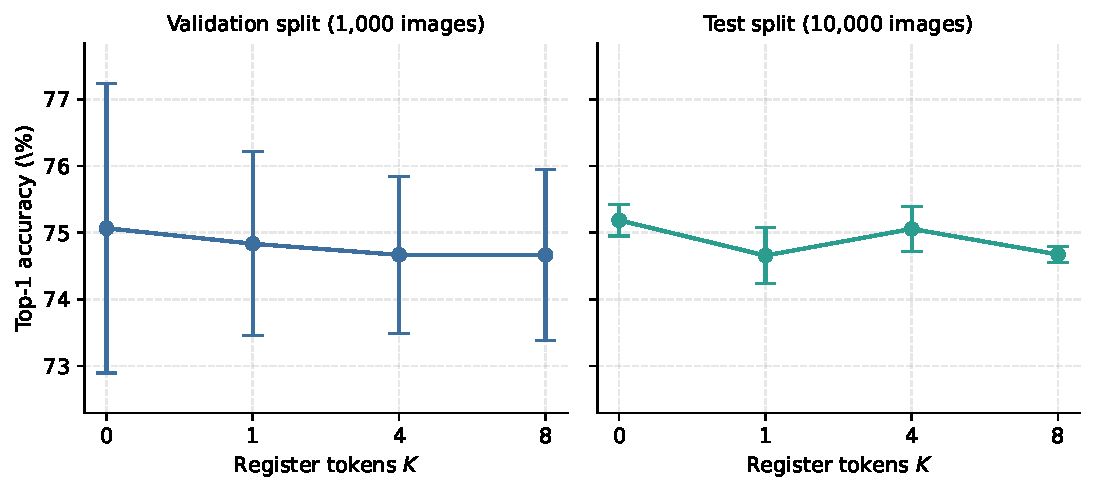
\includegraphics[width=\linewidth]{accuracy_vs_registers.pdf}

\column{0.43\textwidth}
Between-seed spread of Top-1, control arm:

\medskip
\begin{itemize}
\item validation (1{,}000 images): \textbf{2.17 pp}
\item test (10{,}000 images): \textbf{0.24 pp}
\end{itemize}

\medskip
A factor of nine --- and the validation split also selects the
checkpoint.

\medskip
\begin{block}{Methodological takeaway}
A generalization-gap argument built on the split that performs model selection
is not evidence about generalization.
\end{block}
\end{columns}
\end{frame}

\begin{frame}{Result 3: H2 supported at $K=8$, H3 not supported}
\begin{columns}[T]
\column{0.55\textwidth}

\includegraphics[width=\linewidth]{entropy_vs_layer.pdf}

\column{0.43\textwidth}
\textbf{H2 --- capacity dilution.} $K=8$ is the study's only consistent
held-out effect: test loss $+0.0203$, \textbf{3/3} seeds, $p = 0.014$.
Block-12 entropy also falls in 3/3.

\medskip
\textbf{H3 --- entropy collapse.} The four arms lie on top of one another.
Averaged over 12 blocks: $+0.020$, $+0.001$, $-0.025$ bits. None significant.

\medskip
Patch-norm outlier rate: 1.227\%, 1.246\%, 1.250\%, 1.254\%. It rises slightly
with $K$ --- the opposite of the artifact-removal prediction.
\end{columns}
\end{frame}

\begin{frame}{Interpretation: a scope result, not a refutation}
\begin{columns}[T]
\column{0.5\textwidth}
\textbf{Regime mismatch.}
\begin{itemize}
\item Registers were a \emph{pretraining-time} intervention at foundation scale.
\item Ours are randomly initialised into an ImageNet-pretrained backbone and
given 50 epochs over 9{,}000 images.
\item The measured entropy profile of every register arm is the \emph{pretrained}
profile --- the routing never reorganised.
\end{itemize}

\column{0.5\textwidth}
\textbf{The artifacts are real but unmoved.}
\begin{itemize}
\item Control outlier rate 1.23\% $\approx 9\times$ the Gaussian $3\sigma$ rate
of 0.13\%: heavy-tailed structure is present.
\item Registers do not absorb it here.
\end{itemize}

\medskip
\textbf{And $K=8$ is not free.} Eight content-free keys in a 205-token sequence
at $d=192$ measurably cost held-out loss.
\end{columns}
\end{frame}

\begin{frame}{Limits, and what we would run next}
\begin{columns}[T]
\column{0.5\textwidth}
\textbf{Limits we accept}
\begin{itemize}
\item $n = 3$, $\mathrm{df} = 2$; 15 uncorrected comparisons. Direction count is
our primary signal.
\item One architecture, one dataset, one budget.
\item Entropy and outlier rates come from a single 64-image batch --- identical
across all 12 runs, so pairing is sound, but absolute values are estimates.
\item Entropy averages all query rows, not the \texttt{[CLS]} row alone.
\end{itemize}

\column{0.5\textwidth}
\textbf{Next experiment}
\begin{itemize}
\item Pretrain \emph{with} registers at this scale --- the direct test of the
mechanism our design cannot reach.
\item \texttt{[CLS]}-restricted entropy as a sharper H3 instrument.
\item Full-split diagnostic pass rather than one batch.
\end{itemize}

\medskip
The released sweep runner executes all three unchanged.
\end{columns}
\end{frame}

\begin{frame}{Conclusion}
\begin{enumerate}
\item On a low-data CIFAR-100 ViT-Tiny, \textbf{no register configuration
improves held-out accuracy} over the register-free control
($75.19 \pm 0.24\%$).
\item The regularization signature appears on validation
($K=4$: 3/3 seeds, $p = 0.024$) and \textbf{does not transfer} to the test split
($p = 0.823$). Training loss is unchanged, so nothing was regularized.
\item \textbf{$K=8$ costs accuracy and held-out loss} (3/3 seeds, $p = 0.014$),
consistent with capacity dilution at $d = 192$.
\item No evidence for entropy-collapse prevention in either the entropy or the
outlier readout.
\end{enumerate}

\bigskip
\begin{block}{}
Every number here is generated from \texttt{outputs/sweep\_summary.json} by
script. Code, sweep runner and figure generators:
\texttt{github.com/shahin1717/vit-research}
\end{block}
\end{frame}

\end{document}
